%------------------------------------------%
% Cannabis Data Science
% Saturday Morning Statistics
% Date: 2/19/2022
%------------------------------------------%
\documentclass[xcolor={dvipsnames}]{beamer}
\hypersetup{pdfpagemode = FullScreen}
\mode<presentation>{
  \usetheme{Boadilla}
  \usecolortheme{orchid}
  \usefonttheme{default}
  \setbeamertemplate{navigation symbols}{}
  \setbeamertemplate{caption}[numbered]
}
\setbeamersize{
  text margin left = 0.5in,
  text margin right = 0.5in
}

%------------------------------------------%
% Title
%------------------------------------------%
\author{Cannabis Data Science}
\title[\textbf{Saturday Morning Statistics \#13}]{}
\institute[]{\Large Saturday Morning Statistics \#13}
\date{February \nth{19}, 2022}

%------------------------------------------%
% Packages
%------------------------------------------%
\usepackage[english]{babel}
\usepackage[utf8x]{inputenc}
\usepackage{tikz}
\usepackage{xparse}

%------------------------------------------%
% Colors
%------------------------------------------%
\definecolor{Green}{RGB}{34, 153, 84}
\definecolor{LightGreen}{RGB}{218, 247, 166}
\definecolor{DarkGreen}{RGB}{2, 48, 32}
\definecolor{Orange}{RGB}{255, 87, 51}
\definecolor{DarkOrange}{RGB}{199, 0, 57}
\definecolor{Yellow}{RGB}{255, 195, 0}

%------------------------------------------%
% Theme
%------------------------------------------%
\setbeamercolor*{palette primary}{bg=LightGreen, fg=DarkGreen}
\setbeamercolor*{palette secondary}{bg=LightGreen, fg=DarkGreen}
\setbeamercolor*{palette tertiary}{bg=LightGreen, fg=DarkGreen}

%------------------------------------------%
% Packages
%------------------------------------------%
\usepackage{amsmath}
\renewcommand*\footnoterule{} % No separating line on footnote.
\usepackage{mathtools} % For annotating equations.
\usepackage{hhline} % for double bars.
\usepackage[super]{nth} % For formatting 1st, 2nd, 3rd, etc.
\usepackage{graphicx, caption, subcaption}

%------------------------------------------%
% Commands
%------------------------------------------%

% Top space.
\newcommand\T{\rule{0pt}{2.5ex}}

% Bottom space.
\newcommand\B{\rule[-1.25ex]{0pt}{0pt}}

% Blocks.
\newenvironment<>{Block}[2][.9\textwidth]
  {\setlength{\textwidth}{#1}
  \begin{actionenv}#3
    \def\insertblocktitle{#2}\par
    \usebeamertemplate{block begin}}
  {\par\usebeamertemplate{block end}
  \end{actionenv}}

% Balls.
\defbeamertemplate{enumerate item}{largeball}
{\begin{pgfpicture}{-1ex}{-0.65ex}{1.5ex}{1.5ex}
\usebeamercolor[fg]{item projected}
{\pgftransformscale{2.5}\pgftext{\Large\pgfuseshading{bigsphere}}}
{\pgftransformshift{\pgfpoint{0pt}{0.5pt}}
\pgftext{\usebeamerfont*{item projected}\small\insertenumlabel}}
\end{pgfpicture}}

% Fancy arrows.
\NewDocumentCommand\UpArrow{O{2.0ex} O{black}}{%
   \mathrel{\tikz[baseline] \draw [->, line width=0.5pt, #2] (0,0) -- ++(0,#1);}} % Fancy up-arrow.
\NewDocumentCommand\DownArrow{O{2.0ex} O{black}}{%
   \mathrel{\tikz[baseline] \draw [<-, line width=0.5pt, #2] (0,0) -- ++(0,#1);}} % Fancy down-arrow.

% Equations with numbers on the left.
\makeatletter
\newcommand{\LeftEqNo}{\let\veqno\@@leqno}
\makeatother

%------------------------------------------%
% Presentation
%------------------------------------------%
\begin{document}

%------------------------------------------%
% Title Page
%------------------------------------------%
\begin{frame}{}
  
\includegraphics[scale=0.33]{images/logo.pdf}
  \vspace*{-2\baselineskip}
  \titlepage
\end{frame}

%------------------------------------------%
% Prologue
%------------------------------------------%
\begin{frame}{}

% Cholera Map
\begin{figure}
      \caption*{{\bfseries 1854--1858} - A map created by Dr. John Snow (1813-1858) depicting cholera cases in the London epidemics of 1854.}
    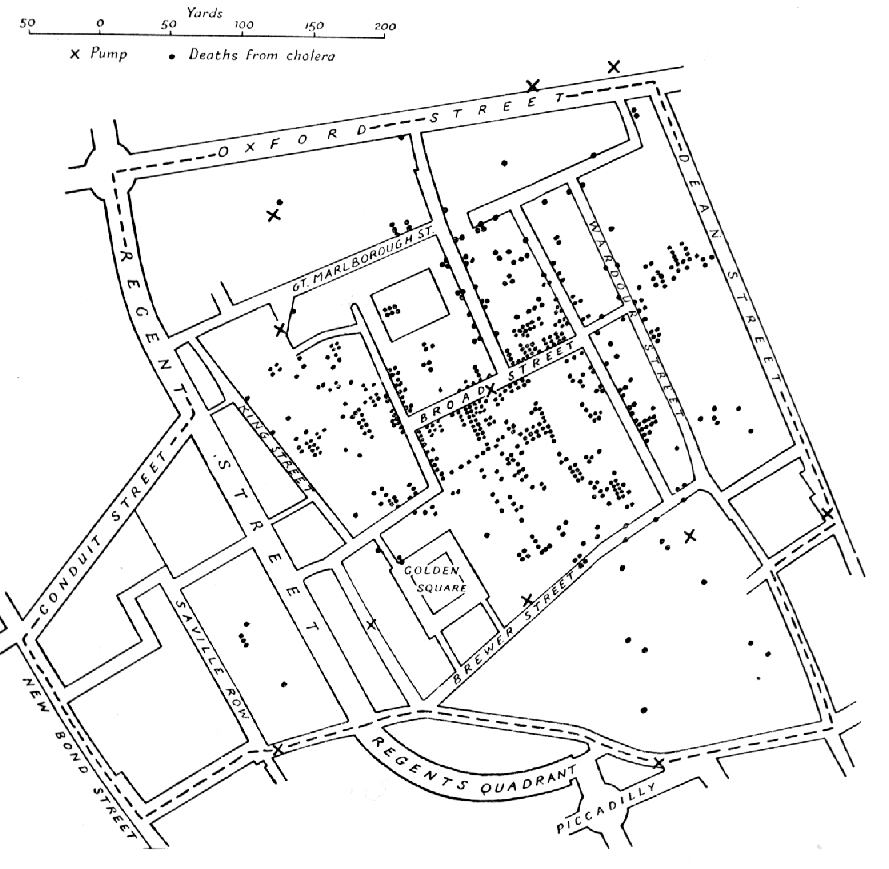
\includegraphics[width=.45\textwidth]{images/john-snow-cholera-map.jpg}
\end{figure}

{\footnotesize {\bfseries Fun fact}: Dr. John Snow's research on cholera gave rise to the modern day difference-in-differences model\textsuperscript{1}.}

\vspace{\baselineskip}

{\tiny Designing Difference in Difference Studies: Best Practices for Public Health Policy Research\vspace{.25\baselineskip}\\Coady Wing et al., (2018).\vspace{-.75\baselineskip}\\https://doi.org/10.1146/annurev-publhealth-040617-013507}

\end{frame}


%------------------------------------------%
% Difference--in--Difference Models
%------------------------------------------%
\section{Difference-in-Differences Models}
\begin{frame}{}

{\large \textbf{Difference--in--Differences Models}}\vspace{.25\baselineskip}\\

\begin{center}
\begin{minipage}{.35\textwidth}
\begin{figure}
    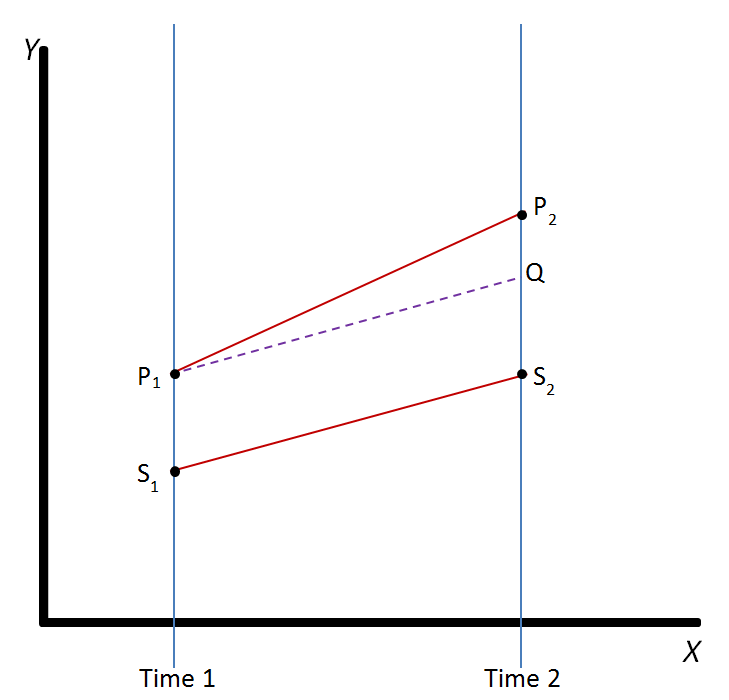
\includegraphics[width=\textwidth]{images/diff-in-diff.png}
    \caption*{\tiny Author: Danni Ruthvan\newline
License: CC BY-SA 3.0 https://creativecommons.org/licenses/by-sa/3.0/deed.en}
\end{figure}
\end{minipage}
\end{center}



{\bfseries Difference--in--differences} techniques can be used to estimate the effects from the causal variable given:

\vspace{\baselineskip}

\begin{enumerate}

\item Panel data;

\vspace{\baselineskip}

\item Certain groups are exposed to a causal variable and others are not.

\end{enumerate}

\end{frame}


% Advantages
\begin{frame}{}

{\large \textbf{Advantages of Difference--in--Differences Models}}\vspace{1\baselineskip}\\

\begin{itemize}

\item Can be used to analyze economic conditions and government policy.

\vspace{\baselineskip}

\item Have been used in hundreds of studies.

\end{itemize}


\vspace{\baselineskip}
Not suitable if:
\vspace{\baselineskip}

\begin{itemize}

\item The composition of groups pre/post change are not stable.

\vspace{\baselineskip}

\item The intervention allocation is determined by the baseline outcome.

\end{itemize}

\end{frame}

% Disadvantages
\begin{frame}{}

{\large \textbf{Disadvantages of Difference--in--Differences Models}}\vspace{.25\baselineskip}\\

\begin{itemize}

\item Requires that in the absence of treatment, the difference between the treatment and control group is constant over time.

\begin{center}
\begin{minipage}{.55\textwidth}
\begin{figure}
    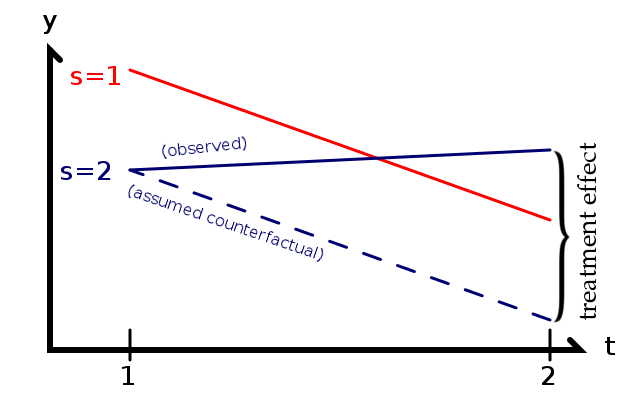
\includegraphics[width=\textwidth]{images/parallel-trend-assumption.png}
    \caption*{\tiny Author: Masalih \newline License: CC BY-SA 3.0 https://creativecommons.org/licenses/by-sa/3.0/deed.en}
\end{figure}
\end{minipage}
\end{center}

\begin{itemize}

\item No statistical test for this assumption;

\vspace{.5\baselineskip}

\item Violation of this assumption will lead to biased estimation of the causal effect.

\end{itemize}

\end{itemize}

\end{frame}


%------------------------------------------%
% Question
%------------------------------------------%
\section{Question}

\begin{frame}{}

\vspace{.5\baselineskip}

\begin{center}
\begin{minipage}{\linewidth}
\begin{Block}{Question of the Day}

\vspace{0.5\baselineskip}
\begin{itemize}

\item Given that we have rich panel data, can we utilize difference--in--differences models to answer any interesting questions? Perhaps...

\begin{itemize}

\vspace{\baselineskip}

\item What effect, if any, did the temporary closure of retail in Massachusetts in April of 2020 have on prices?

\vspace{\baselineskip}

\item Any of your ideas?

\end{itemize}

\end{itemize}

\vspace{0.25\baselineskip}

\end{Block}
\end{minipage}
\end{center}

\vfill

\end{frame}


%------------------------------------------%
% Classical Linear Regression
%------------------------------------------%
\section{The Classical Linear Regressions}
\begin{frame}{}

{\large \textbf{The Classical Linear Regressions}}\vspace{\baselineskip}\\

A linear equation with $n$ independent variables:

$$y = \beta_0 + \beta_1 x_1 + ... + \beta_n x_n + \epsilon$$
\vspace{.125\baselineskip}\\

In matrix notation:

$$y = \beta^TX + \epsilon$$
\vspace{.125\baselineskip}\\

With closed form solution:

$$\hat{\beta} = (X^TX)^{-1}X^Ty$$

\end{frame}

%------------------------------------------%
% The Bayesian Approach to Linear Regressions
%------------------------------------------%
\section{The Bayesian Approach to Linear Regressions}
\begin{frame}{}

{\large \textbf{The Bayesian Approach to Linear Regressions}}\vspace{\baselineskip}\\

The data is assumed to be sampled from a distribution:

$$y \sim N(\beta^TX, \sigma^2I)$$
\vspace{.125\baselineskip}\\

The posterior probability is:

$$P(\beta | y, X) = \frac{P(y|\beta,X)\times P(\beta | X)}{P(y | X)}$$
\vspace{.125\baselineskip}\\

Essentially:

$$\text{Posterior} = \frac{\text{Likelihood}\times\text{Prior}}{\text{Normalization}}$$

\end{frame}


%------------------------------------------%
% Takeaway
%------------------------------------------%
\section{Takeaway}
\begin{frame}{}

\begin{center}
\begin{minipage}{3.85in}

% Thank you.
\begin{center}

\includegraphics[width=.25in]{images/prayer.png} {\Large \textbf{Thank you for coming.}}\\
\end{center}

% Re-cap the lesson of the week.
\begin{center}
\begin{minipage}{\linewidth}
\begin{Block}{Lesson of the Day}

\vspace{0.5\baselineskip}

\begin{itemize}

\item Assumptions matter.

\vspace{0.5\baselineskip}

\end{itemize}

\end{Block}
\end{minipage}
\end{center}

\vfill

\end{minipage}
\end{center}

\end{frame}

% References

% https://www.sciencedirect.com/topics/economics-econometrics-and-finance/difference-in-differences


%------------------------------------------%
% End
%------------------------------------------%
\end{document}
